\chapter{Does Pleasure Bring Happiness?}

This chapter follows J. Krishnamurti's dialogue with Dr. Alan W. Anderson on pleasure, enjoyment, joy, happiness, thought, attention, discipline, and freedom. There is no blackboard mathematics in the source material, so the displayed formulae and diagrams in this chapter are not recovered equations. They are compact, transcript-based schemata: a disciplined way of preserving the order of the inquiry without turning it into doctrine or self-help.

\section{The Question Pleasure Cannot Evade}

Anderson begins by returning to the previous movement of the conversations. The inquiry has passed through fear and arrived at pleasure. Now the words begin to multiply: pleasure, enjoyment, delight, joy, happiness. The first temptation is to assume that these names form a family, perhaps a scale, perhaps a gentle ascent from ordinary pleasure to some more refined happiness.

Krishnamurti interrupts that assumption. The question is not whether English usage sometimes lets pleasure lean toward joy. The question is whether, in fact, there is a line of continuity between them. We can write the opening uncertainty as a deliberately unresolved map:
\begin{equation}
\text{pleasure} \quad ? \quad \text{enjoyment} \quad ? \quad \text{joy} \quad ? \quad \text{happiness}.
\end{equation}
The question mark matters. The whole lecture turns on refusing to let ordinary usage settle the matter.

Anderson notices the word ``please.'' To say ``please sit down'' may carry the trace of being pleased, of invitation, of pleasure. Krishnamurti hears the linguistic point but does not stay with it. He asks instead whether there is, beyond the word, any actual connecting link:
\begin{equation}
\text{pleasure} \longrightarrow \text{joy} \quad ?
\end{equation}
The arrow is not yet asserted. It is under examination.

\subsection{Question \& Answer}

\paragraph{Question.}
Is pleasure a continuation of joy, or a lower form of joy, or a movement that can eventually become happiness?

\paragraph{Answer.}
Krishnamurti's inquiry begins by suspending that assumption. Pleasure may share vocabulary with enjoyment and joy, but the lecture will test whether pleasure has its own structure. The first task is therefore not to define joy, but to ask what pleasure is and what keeps it going.

\section{Pleasure As Pursuit And Possession}

Krishnamurti does not define pleasure by choosing a noble example. He lists ordinary pleasures and disturbing pleasures together: eating, walking, accumulating money, sex, hurting people, power, possession, knowledge, religious ideas, and political domination. The point is severe but precise. Pleasure is not made innocent or corrupt by its object alone. It must be understood by its movement.

The common structure is that pleasure is sustained, nourished, and kept going:
\begin{equation}
\text{pleasure} = \text{a movement sustained by thought in a direction}.
\end{equation}
This is a conceptual formula, not a psychological law. It preserves Krishnamurti's emphasis that pleasure has direction. It moves toward having, repeating, continuing, enlarging, or protecting something.

The examples of possession clarify the matter. A child has pleasure in a toy; an adult in a house; a scholar in knowledge; a religious mind in the idea of God; a dictator in power. The objects differ, but the movement has a recognizable form:
\begin{align}
\text{object seen or held} &\longrightarrow \text{wanting it},\\
\text{wanting it} &\longrightarrow \text{possession},\\
\text{possession} &\longrightarrow \text{pleasure sustained}.
\end{align}
When that movement is blocked, the lecture gives a second chain:
\begin{equation}
\text{thwarted pleasure}
\longrightarrow
\text{frustration}
\longrightarrow
\text{anger, jealousy, violence}.
\end{equation}
Again, the notation is a guide to order. It is not a claim that every instance follows a mechanical rule. It records the relation Krishnamurti is drawing: pursued pleasure, when denied, is not neutral. It becomes conflict.

\section{The Tree, Memory, And Repetition}

To make the structure simple, Krishnamurti turns to a scene: a single tree on a hill, a green meadow, water, deer, flowers, shadow. One sees it. There is an immediate response. It is not yet romantic, sentimental, verbal, or possessed. It is simply perception.

Then one turns away. Thought enters and says, in effect: how extraordinary that was. I must have it again. Here the lecture gives its central derivation.

\paragraph{Worked reconstruction.}
We can reconstruct the movement in five steps:
\begin{enumerate}
\item There is direct perception of beauty.
\item Thought remembers the perception.
\item Memory carries the perception forward as an image.
\item Desire demands the repetition of the image.
\item The pursuit of that repetition becomes pleasure.
\end{enumerate}
In compact form:
\begin{equation}
\text{perception}
\longrightarrow
\text{thought}
\longrightarrow
\text{memory}
\longrightarrow
\text{repetition}
\longrightarrow
\text{pursuit}.
\end{equation}

The decisive point is that Krishnamurti does not call the first perception pleasure. In the moment of seeing the tree, the hill, the water, and the shadow, there is perception. Pleasure arises when thought returns to the perception and demands its continuation.

\begin{figure}
\centering
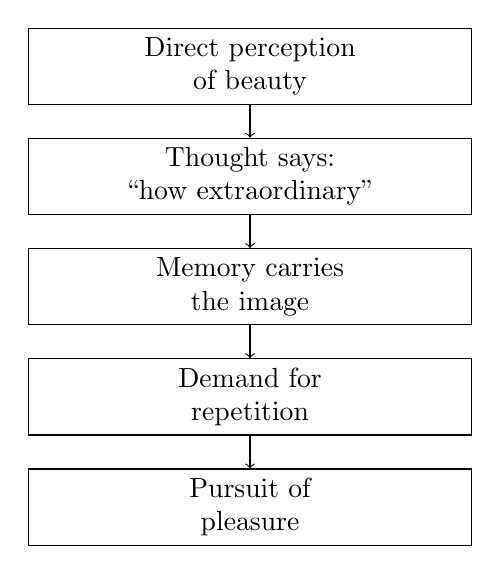
\begin{tikzpicture}[x=1cm,y=1cm]
\node[draw, text width=5.4cm, align=center] (a) at (0,0) {Direct perception\\of beauty};
\node[draw, text width=5.4cm, align=center] (b) at (0,-1.4) {Thought says:\\``how extraordinary''};
\node[draw, text width=5.4cm, align=center] (c) at (0,-2.8) {Memory carries\\the image};
\node[draw, text width=5.4cm, align=center] (d) at (0,-4.2) {Demand for\\repetition};
\node[draw, text width=5.4cm, align=center] (e) at (0,-5.6) {Pursuit of\\pleasure};
\draw[->] (a) -- (b);
\draw[->] (b) -- (c);
\draw[->] (c) -- (d);
\draw[->] (d) -- (e);
\end{tikzpicture}

Transcript-based reconstruction of the movement from perception to the pursuit of pleasure.
\end{figure}

Anderson's examples of encore and festival widen the point. Repetition is not merely private. Culture can organize itself around the attempt to repeat intensity. What began as one movement of thought becomes a social rhythm: the encore, the festival, the effort to ``live it up,'' followed by the ordinary descent back into routine.

\section{Enjoyment, Joy, And The Movement Of Thought}

The lecture now returns to the opening question. If pleasure is thought moving in a direction, what is its relation to enjoyment, delight, joy, and happiness?

Krishnamurti's answer is compressed and exact:
\begin{equation}
\text{enjoyment}
+
\text{thought}(\text{``I must have more''})
\longrightarrow
\text{pleasure}.
\end{equation}
Enjoyment becomes pleasure when thought appropriates it and demands continuation. Joy and happiness are not invited in this way. They are not summoned by demand, directed by memory, or held through repetition. One may say afterward that there was happiness, but in the moment itself the self-conscious claim is absent.

\begin{table}
\centering
\begin{tabular}{|p{0.24\linewidth}|p{0.62\linewidth}|}
\hline
\textbf{Term} & \textbf{Working distinction in the dialogue} \\
\hline
Pleasure & Thought-sustained movement in a direction; linked to repetition and pursuit. \\
\hline
Enjoyment & Immediate enjoyment; becomes pleasure when thought demands more. \\
\hline
Delight & A direct, inexpressible freshness, not yet organized by pursuit. \\
\hline
Joy & Not invited, not repeated by will, not a continuity of pleasure. \\
\hline
Happiness & Not known as an object while it is present; named only afterward. \\
\hline
\end{tabular}

Transcript-based distinction among the central terms.
\end{table}

\subsection{Question \& Answer}

\paragraph{Question.}
When does enjoyment become pleasure?

\paragraph{Answer.}
Enjoyment becomes pleasure when thought says, ``I have enjoyed it; I must have more of it.'' The change is not in the original seeing or enjoying, but in the entry of memory, image, demand, and direction.

\paragraph{Question.}
Does pleasure therefore have a relation to joy or happiness?

\paragraph{Answer.}
In this dialogue, no continuity is granted. Pleasure belongs to the movement of thought in a direction. Joy and happiness are not produced by that movement. They are not invited, accumulated, or repeated.

\section{Attention Instead Of Control}

The next question arises naturally. If thought enters enjoyment and converts it into pleasure, should thought be controlled? Krishnamurti presents the traditional answer: religious discipline has often meant controlling thought, cutting it off when it rises, suppressing it before it interferes.

But he rejects that solution. Control is still division. It is still conflict. It is still thought acting on thought. We can mark the rejected path as:
\begin{equation}
\text{thought interferes}
\longrightarrow
\text{control thought}
\longrightarrow
\text{suppression and conflict}.
\end{equation}
The alternative is not negligence. It is attention. When one sees wholly, thought does not creep in. Anderson clarifies that this is not muscular effort, not tightening oneself in concentration. Krishnamurti's phrase is simpler: be wholly there.

Thus the structure becomes:
\begin{equation}
\text{complete attention}
\longrightarrow
\text{no interference of thought}
\longrightarrow
\text{action without control}.
\end{equation}

\subsection{Question \& Answer}

\paragraph{Question.}
If thought turns enjoyment into the pursuit of pleasure, must thought be controlled?

\paragraph{Answer.}
No. Control is part of the same divided movement. Krishnamurti's answer is complete attention. In such attention, thought does not enter as the demand to repeat. This is not a method of concentration and not a cultivated technique.

The poisonous bottle example gives the practical form of this point. If one really sees that the bottle is poisonous, one does not need to control the desire to drink it. Seeing is already action. Control is necessary only when the thing has not been read clearly.

Krishnamurti then gives one of the central compressed statements of the lecture:
\begin{equation}
\text{watching} \equiv \text{discipline} \equiv \text{action}.
\end{equation}
The equivalence sign is only a notation for the spoken compression. It should not be read as formal identity. The meaning is that watching, when it is actual, is not a preliminary to discipline or action. It is already disciplined action.

\begin{figure}
\centering
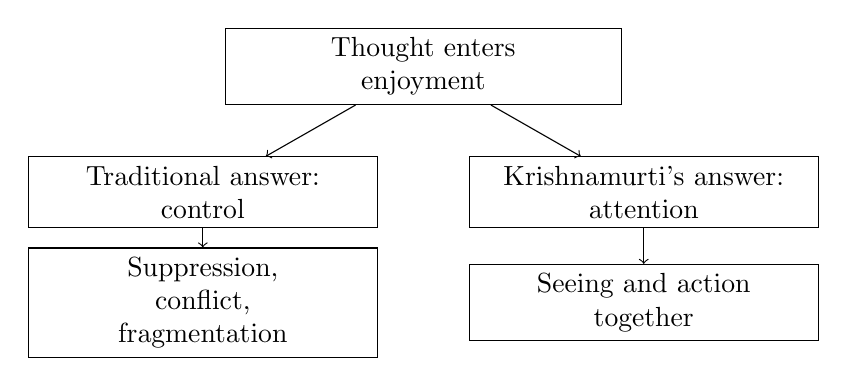
\begin{tikzpicture}[x=1cm,y=1cm]
\node[draw, text width=4.8cm, align=center] (root) at (0,0) {Thought enters\\enjoyment};

\node[draw, text width=4.2cm, align=center] (c1) at (-2.8,-1.6) {Traditional answer:\\control};
\node[draw, text width=4.2cm, align=center] (c2) at (-2.8,-3.0) {Suppression,\\conflict,\\fragmentation};

\node[draw, text width=4.2cm, align=center] (a1) at (2.8,-1.6) {Krishnamurti's answer:\\attention};
\node[draw, text width=4.2cm, align=center] (a2) at (2.8,-3.0) {Seeing and action\\together};

\draw[->] (root) -- (c1);
\draw[->] (c1) -- (c2);
\draw[->] (root) -- (a1);
\draw[->] (a1) -- (a2);
\end{tikzpicture}

Transcript-based reconstruction of the contrast between control and attention.
\end{figure}

\section{Intelligence Without Possession}

Anderson then presses a subtle question. If attention acts without control, if watching has its own discipline, is there some abiding support behind it? Is there something permanent, some inner source, sustaining the person?

Krishnamurti refuses the formulation. It opens the door to God, higher self, Atman, or a permanent entity inside the person. The refusal is important because it prevents the inquiry from becoming metaphysical consolation. Intelligence is not a possession. It is not something one has and then permits to operate.

The safer reconstruction is:
\begin{equation}
\text{observation} + \text{attention} + \text{careful seeing}
\longrightarrow
\text{intelligence}.
\end{equation}
Even here the arrow must be read carefully. It does not mean that observation is a technique that manufactures intelligence. It means that, in the act of seeing, intelligence is present.

\subsection{Question \& Answer}

\paragraph{Question.}
Is intelligence an inner support, a higher self, or a permanent source within the person?

\paragraph{Answer.}
Krishnamurti rejects that language. To say that there is an abiding support risks making intelligence into a doctrine or possession. In this dialogue, intelligence comes in observation. It is sensitivity in seeing, not a metaphysical object.

This also explains why the lecture refuses the idea that one must pass through every experience in order to understand it. Krishnamurti asks, in effect: must one get drunk to see the movement of drunkenness? The answer is no. One can observe the whole movement without becoming it. Seeing is not accumulation of experience; it is direct perception of structure.

\section{Discipline Means Learning}

After the refusal of control and possession, the word discipline must be rebuilt. In ordinary religious or moral language, discipline often means conformity, suppression, adjustment to a pattern, or obedience to a method. Krishnamurti returns the word to learning.

The corrected relation is:
\begin{equation}
\text{discipline} = \text{learning}.
\end{equation}
Learning here is not accumulation of information. It is the active capacity to hear, to see, to observe. Krishnamurti distinguishes cultivated capacity from the act of listening. A capacity may be developed through time; perception, in the sense he is using the word, is immediate.

We may record the distinction as:
\begin{align}
\text{cultivated capacity} &\sim \text{time},\\
\text{perception} &\not\sim \text{time}.
\end{align}
This is not physics notation. It is a compact way to preserve the difference in the transcript: practice may require duration, but perception is not perfected at the end of practice.

Anderson sees the implication: there has been a confusion between perception and practice, as though perception were perfected at the end of training. Krishnamurti reverses that. Freedom is not at the end; it is at the beginning. The first step counts.

The relation between seeing, learning, and acting is therefore simultaneous:
\begin{equation}
\text{seeing} \;+\; \text{learning} \;+\; \text{acting}
\quad \text{occur together}.
\end{equation}
This is the point at which the lecture links discipline to order. Learning about pleasure brings its own order. It is not imposed order. It is not the order of control. It is the order that comes when the movement has been read.

\begin{figure}
\centering
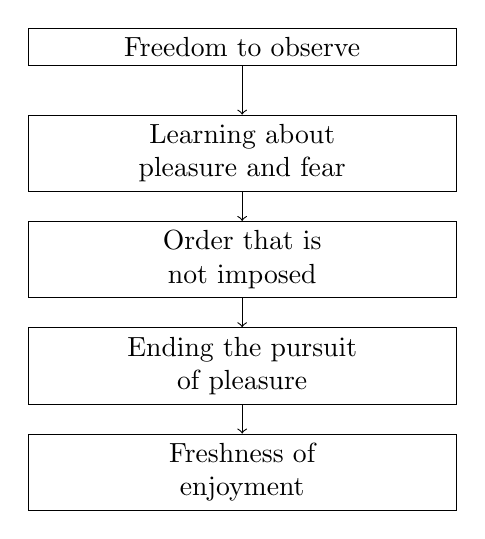
\begin{tikzpicture}[x=1cm,y=1cm]
\node[draw, text width=5.2cm, align=center] (a) at (0,0) {Freedom to observe};
\node[draw, text width=5.2cm, align=center] (b) at (0,-1.35) {Learning about\\pleasure and fear};
\node[draw, text width=5.2cm, align=center] (c) at (0,-2.7) {Order that is\\not imposed};
\node[draw, text width=5.2cm, align=center] (d) at (0,-4.05) {Ending the pursuit\\of pleasure};
\node[draw, text width=5.2cm, align=center] (e) at (0,-5.4) {Freshness of\\enjoyment};
\draw[->] (a) -- (b);
\draw[->] (b) -- (c);
\draw[->] (c) -- (d);
\draw[->] (d) -- (e);
\end{tikzpicture}

Transcript-based reconstruction of learning as order.
\end{figure}

Krishnamurti also distinguishes conditioned reaction from perception-action. A person sees a physical danger and reacts instantly because the organism is conditioned to protect itself. That conditioning is not intelligence. The deeper claim is different: perception and action, when the mind sees clearly, are not conditioned responses. They occur together because the seeing is complete.

\section{Attention, Care, And The Whole Map}

Near the end, the lecture broadens again. Attention is not something to be practiced, cultivated, or learned from a school. To seek a method of attention is already to miss attention. Attention includes care, affection, diligence, and the capacity to read exactly what is there without interpretation.

This returns us to the title question. Does pleasure bring happiness? The answer, in the terms of this dialogue, is no. Pleasure as pursuit is thought moving in a direction. It repeats, substitutes, becomes bored, seeks new directions, and may become violent when denied. Happiness and joy are not products of that movement.

The dialogue's wider map can be drawn in the order Krishnamurti recalls:
\begin{figure}
\centering
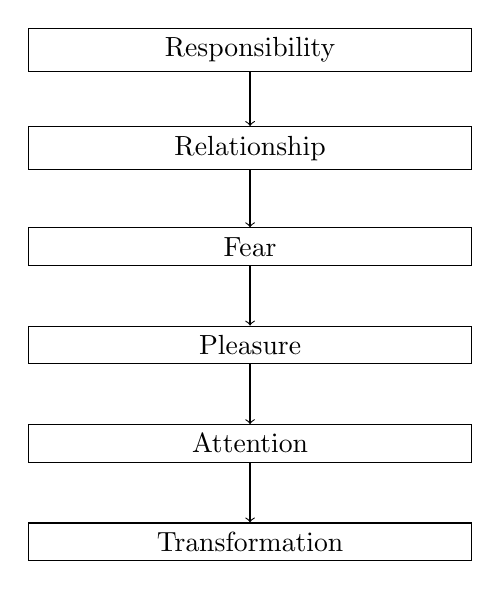
\begin{tikzpicture}[x=1cm,y=1cm]
\node[draw, text width=5.4cm, align=center] (r) at (0,0) {Responsibility};
\node[draw, text width=5.4cm, align=center] (rel) at (0,-1.25) {Relationship};
\node[draw, text width=5.4cm, align=center] (f) at (0,-2.5) {Fear};
\node[draw, text width=5.4cm, align=center] (p) at (0,-3.75) {Pleasure};
\node[draw, text width=5.4cm, align=center] (att) at (0,-5.0) {Attention};
\node[draw, text width=5.4cm, align=center] (tr) at (0,-6.25) {Transformation};
\draw[->] (r) -- (rel);
\draw[->] (rel) -- (f);
\draw[->] (f) -- (p);
\draw[->] (p) -- (att);
\draw[->] (att) -- (tr);
\end{tikzpicture}

The lecture's recap of the inquiry as a map of life.
\end{figure}

The final movement is quiet but important. Krishnamurti speaks of reading the whole map of life: responsibility, relationship, fear, pleasure, and the rest. Anderson recognizes that the inquiry has stayed within the question of the transformation of man without needing to force a system. The transformation is not dependent on knowledge or time. It is bound to seeing.

The chapter should therefore leave pleasure where the lecture leaves it: not condemned, not indulged, not denied, but understood. Enjoyment can end as it happens. Pleasure becomes bondage when it is carried over, repeated, and pursued. Attention reads the movement as it occurs.

\section{Summary}

The lecture begins with a question about language and ends with a map of life. Its central distinction is that pleasure is not the same as enjoyment, joy, or happiness. Pleasure begins when thought takes an immediate perception or enjoyment and turns it into memory, repetition, demand, and pursuit.

The main structure is:
\begin{equation}
\text{perception}
\longrightarrow
\text{thought}
\longrightarrow
\text{memory}
\longrightarrow
\text{repetition}
\longrightarrow
\text{pleasure as pursuit}.
\end{equation}
The answer is not control. Control belongs to division and suppression. The alternative is complete attention, in which seeing and action are not separated:
\begin{equation}
\text{attention}
\longrightarrow
\text{seeing and action together}.
\end{equation}
From this, discipline receives a different meaning. It is not conformity to a pattern. It is learning. And when the mind learns the structure of pleasure, that learning brings its own order.